% Created 2012-07-20 Fri 21:00
\documentclass[12pt]{article}
\usepackage[utf8]{inputenc}
\usepackage[T1]{fontenc}
\usepackage{fixltx2e}
\usepackage{graphicx}
\usepackage{longtable}
\usepackage{float}
\usepackage{wrapfig}
\usepackage{soul}
\usepackage{textcomp}
\usepackage{marvosym}
\usepackage{wasysym}
\usepackage{latexsym}
\usepackage{amssymb}
\usepackage{hyperref}
\tolerance=1000
\usepackage[paperwidth=8.5in,paperheight=11in]{geometry}
\geometry{verbose,tmargin=0.5in,bmargin=1in,lmargin=1in,rmargin=1in}
\providecommand{\alert}[1]{\textbf{#1}}

\title{Fitting Nonseasonal ARIMA Models with \texttt{R}}
%\author{G. Jay Kerns}
\date{\vspace{-0.5in}STAT 5848/6948: Applied Regression and Time Series}
\hypersetup{
  pdfkeywords={},
  pdfsubject={},
  pdfcreator={Emacs Org-mode version 7.8.10}}

\begin{document}

\maketitle


For each of the models below we simulate some data according to the model, plot the data, fit the model with \texttt{R}, and show where the parameter estimates would go in the model formula.  We use the \texttt{Arima} function from the \texttt{forecast} package\footnote{We could use the \texttt{arima} function (notice, lowercase) in base \texttt{R} instead and \emph{almost} all of the code would work without change.  The only difference would be the $ARIMA$ models with differencing and nonzero drift, because the ordinary \texttt{arima} function does not have an \texttt{include.drift} argument.  Indeed, it turns out to be quite tricky to estimate a drift with base \texttt{arima}; see \href{http://www.stat.pitt.edu/stoffer/tsa3/Rissues.htm}{here} for a discussion and examples.
 } to estimate the parameters.



\section*{$MA(3)$ with zero mean}
\label{sec-1}


\begin{verbatim}
y <- arima.sim(model = list(ma = c(0.3, 0.2, 0.1)), n = 100)
\end{verbatim}





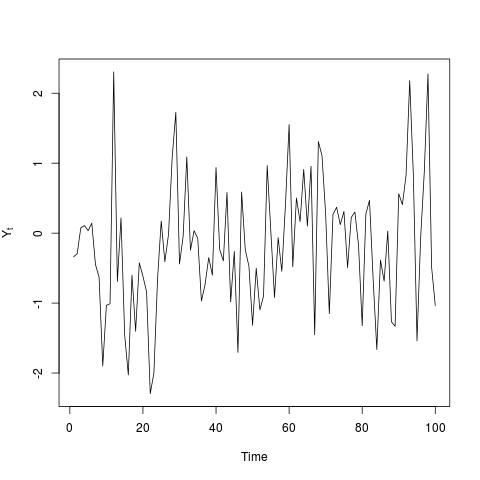
\includegraphics[width=4.0in]{img/ma3zm.png}

\noindent
\textbf{The Theoretical Model:} 
\[
Y_{t} = e_{t} + \theta_{1}e_{t - 1} + \theta_{2}e_{t - 2} + \theta_{3}e_{t - 3},\ t = 1,2,\ldots
\]

\noindent
\textbf{How to Fit the Model with R:}

\begin{verbatim}
Arima(y, order = c(0,0,3), include.mean = FALSE)
\end{verbatim}




\begin{verbatim}
Series: y 
ARIMA(0,0,3) with zero mean     

Coefficients:
         ma1     ma2      ma3
      0.2485  0.0809  -0.0584
s.e.  0.0999  0.0950   0.0880

sigma^2 estimated as 0.8372:  log likelihood=-133.05
AIC=274.1   AICc=274.53   BIC=284.53
\end{verbatim}

\noindent
\textbf{The Fitted Model:} 
\[
Y_{t} = e_{t} + 0.2485 e_{t - 1} + 0.0809 e_{t - 2} + -0.0584 e_{t - 3},\ t = 1,2,\ldots
\]
\section*{$AR(2)$ with zero mean}
\label{sec-2}


\begin{verbatim}
y <- arima.sim(model = list(ar = c(0.3, 0.2)), n = 100)
\end{verbatim}





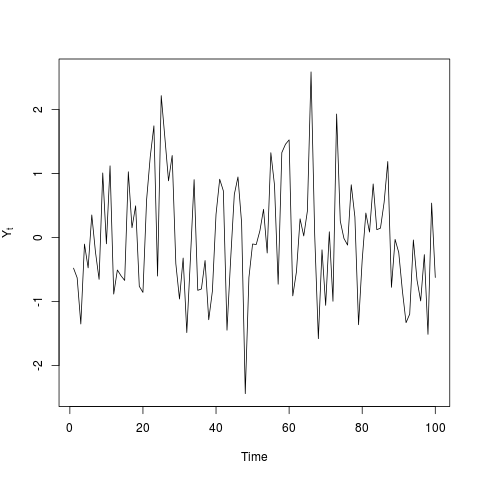
\includegraphics[width=4.0in]{img/ar2zm.png}

\noindent
\textbf{The Theoretical Model:} 
\[
Y_{t} = \phi_{1}Y_{t - 1} + \phi_{2}Y_{t - 2}  + e_{t},\ t = 1,2,\ldots
\]

\noindent
\textbf{How to Fit the Model with R:}


\begin{verbatim}
Arima(y, order = c(2,0,0), include.mean = FALSE)
\end{verbatim}




\begin{verbatim}
Series: y 
ARIMA(2,0,0) with zero mean     

Coefficients:
         ar1      ar2
      0.1924  -0.0088
s.e.  0.0999   0.0998

sigma^2 estimated as 0.8214:  log likelihood=-132.07
AIC=270.15   AICc=270.4   BIC=277.97
\end{verbatim}

\noindent
\textbf{The Fitted Model:} 
\[
Y_{t} = 0.1924 Y_{t - 1} + -0.0088 Y_{t - 2}  +  e_{t},\ t = 1,2,\ldots
\]
\section*{$MA(3)$ with non-zero mean}
\label{sec-3}


\begin{verbatim}
y <- 5 + arima.sim(model = list(ma = c(0.3, 0.2, 0.1)), n = 100)
\end{verbatim}





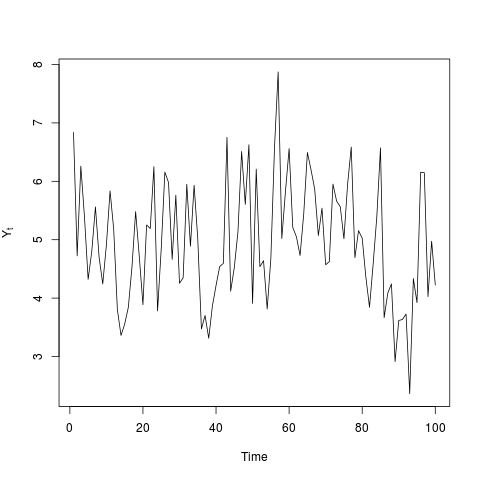
\includegraphics[width=4.0in]{img/ma3nzm.png}

\noindent
\textbf{The Theoretical Model:} 
\[
(Y_{t} - \mu) = e_{t} + \theta_{1}e_{t - 1} + \theta_{2}e_{t - 2} + \theta_{3}e_{t - 3},\ t = 1,2,\ldots
\]

\noindent
\textbf{How to Fit the Model with R:}

\begin{verbatim}
Arima(y, order = c(0,0,3))
\end{verbatim}





\begin{verbatim}
Series: y 
ARIMA(0,0,3) with non-zero mean 

Coefficients:
         ma1     ma2     ma3  intercept
      0.3058  0.1650  0.0440     4.9656
s.e.  0.1011  0.0972  0.0922     0.1440

sigma^2 estimated as 0.9129:  log likelihood=-137.4
AIC=284.8   AICc=285.44   BIC=297.82
\end{verbatim}

\noindent
\textbf{The Fitted Model:} 
\[
(Y_{t} - 4.9656) = e_{t} + 0.3058 e_{t - 1} + 0.165 e_{t - 2} + 0.044 e_{t - 2},\ t = 1,2,\ldots
\]
that is,
\[
Y_{t} = 4.9656 + e_{t} + 0.3058 e_{t - 1} + 0.165 e_{t - 2} + 0.044 e_{t - 3},\ t = 1,2,\ldots
\]
\section*{$AR(2)$ with non-zero mean}
\label{sec-4}


\begin{verbatim}
y <- 21 +  arima.sim(model = list(ar = c(0.3, 0.2)), n = 100)
\end{verbatim}





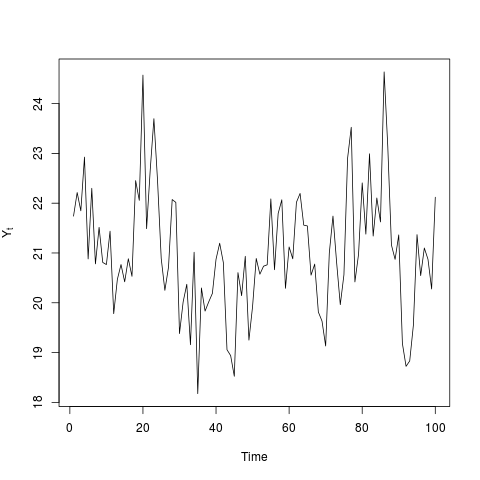
\includegraphics[width=4.0in]{img/ar2nzm.png}

\noindent
\textbf{The Theoretical Model:} 
\[
(Y_{t} - \mu) = \phi_{1}(Y_{t - 1} - \mu) + \phi_{2}(Y_{t - 2} - \mu) + e_{t},\ t = 1,2,\ldots
\]

\noindent
\textbf{How to Fit the Model with R:}


\begin{verbatim}
Arima(y, order = c(2,0,0))
\end{verbatim}




\begin{verbatim}
Series: y 
ARIMA(2,0,0) with non-zero mean 

Coefficients:
         ar1     ar2  intercept
      0.3926  0.1709    21.0322
s.e.  0.0986  0.0990     0.2391

sigma^2 estimated as 1.125:  log likelihood=-147.92
AIC=303.85   AICc=304.27   BIC=314.27
\end{verbatim}

\noindent
\textbf{The Fitted Model:} 
\[
(Y_{t} - 21.0322 ) = 0.3926 (Y_{t - 1} - 21.0322 ) + 0.1709 (Y_{t - 2} - 21.0322 ) + e_{t},\ t = 1,2,\ldots
\]
that is,
\[
Y_{t} =  9.1806 + 0.3926 Y_{t - 1} + 0.1709 Y_{t - 2} + e_{t},\ t = 1,2,\ldots
\]
\section*{$ARMA(1,2)$ with zero mean}
\label{sec-5}


\begin{verbatim}
y <- arima.sim(model = list(ar = 0.8, ma = c(0.7, 0.6)), n = 189)
\end{verbatim}





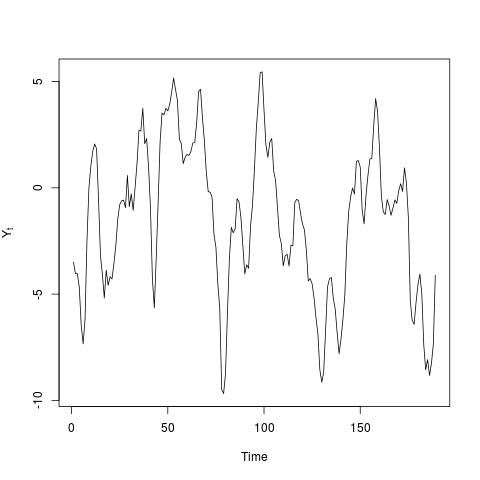
\includegraphics[width=4.0in]{img/arma12zm.png}

\noindent
\textbf{The Theoretical Model:} 
\[
Y_{t} = \phi Y_{t - 1} + e_{t} + \theta_{1} e_{t - 1} + \theta_{2} e_{t - 2},\ t = 1,2,\ldots
\]

\noindent
\textbf{How to Fit the Model with R:}


\begin{verbatim}
Arima(y, order = c(1,0,2), include.mean = FALSE)
\end{verbatim}




\begin{verbatim}
Series: y 
ARIMA(1,0,2) with zero mean     

Coefficients:
         ar1     ma1     ma2
      0.8460  0.6769  0.5891
s.e.  0.0408  0.0700  0.0631

sigma^2 estimated as 0.9312:  log likelihood=-263.29
AIC=534.59   AICc=534.8   BIC=547.55
\end{verbatim}

\noindent
\textbf{The Fitted Model:} 
\[
Y_{t} = 0.846 Y_{t - 1} + e_{t} + 0.6769 e_{t - 1} + 0.5891 e_{t - 1},\ t = 1,2,\ldots
\]
\section*{$ARMA(1,2)$ with non-zero mean}
\label{sec-6}


\begin{verbatim}
y <- 11 + arima.sim(model = list(ar = 0.8, ma = c(0.7, 0.6)), n = 189)
\end{verbatim}





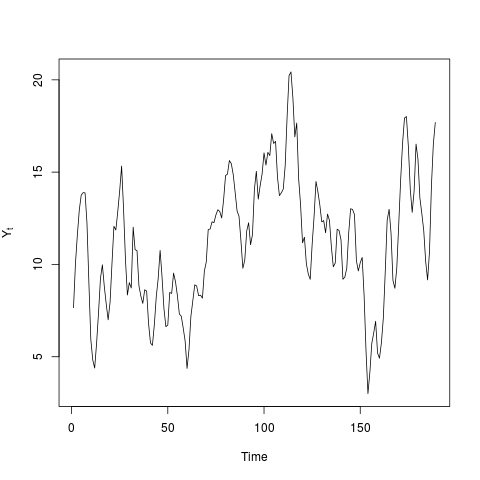
\includegraphics[width=4.0in]{img/arma12nzm.png}

\noindent
\textbf{The Theoretical Model:} 
\[
(Y_{t} - \mu) = \phi(Y_{t - 1} - \mu) +  e_{t} + \theta_{1} e_{t - 1} + \theta_{2} e_{t - 2},\ t = 1,2,\ldots
\]

\noindent
\textbf{How to Fit the Model with R:}


\begin{verbatim}
Arima(y, order = c(1,0,2))
\end{verbatim}




\begin{verbatim}
Series: y 
ARIMA(1,0,2) with non-zero mean 

Coefficients:
         ar1     ma1     ma2  intercept
      0.7648  0.7631  0.6239    11.2171
s.e.  0.0520  0.0582  0.0713     0.7726

sigma^2 estimated as 1.143:  log likelihood=-282.55
AIC=575.09   AICc=575.42   BIC=591.3
\end{verbatim}

\noindent
\textbf{The Fitted Model:} 
\[
(Y_{t} - 11.2171 ) = 0.7648 (Y_{t - 1} - 11.2171 ) + e_{t} + 0.7631 e_{t - 1} + 0.6239 e_{t - 2},\ t = 1,2,\ldots
\]
that is,
\[
Y_{t} = 2.6383 + 0.7648 Y_{t - 1} + e_{t} + 0.7631 e_{t - 1} + 0.6239 e_{t - 2},\ t = 1,2,\ldots
\]
\section*{ARIMA(1,1,2) without drift}
\label{sec-7}


\begin{verbatim}
ydiff <- arima.sim(model = list(ar = 0.8, ma = c(0.7, 0.6)), n = 196)
y <- ts(cumsum(ydiff))
\end{verbatim}





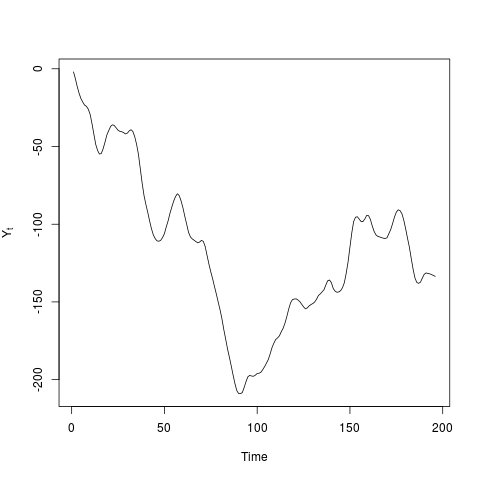
\includegraphics[width=4.0in]{img/arima112zm.png}

\noindent
\textbf{The Theoretical Model:} 
\[
\nabla Y_{t} = \phi \nabla Y_{t - 1} +  e_{t} + \theta_{1} e_{t - 1} + \theta_{2} e_{t - 2},\ t = 1,2,\ldots
\]

\noindent
\textbf{How to Fit the Model with R:}


\begin{verbatim}
Arima(y, order = c(1,1,2))
\end{verbatim}




\begin{verbatim}
Series: y 
ARIMA(1,1,2)                    

Coefficients:
         ar1     ma1     ma2
      0.8177  0.6787  0.6349
s.e.  0.0425  0.0547  0.0601

sigma^2 estimated as 0.9312:  log likelihood=-271.59
AIC=551.18   AICc=551.39   BIC=564.27
\end{verbatim}

\noindent
\textbf{The Fitted Model:} 
\[
\nabla Y_{t} = 0.8177 \nabla Y_{t - 1} + e_{t} + 0.6787 e_{t - 1} + 0.6349 e_{t - 2},\ t = 1,2,\ldots
\]
\section*{ARIMA(1,1,2) with drift}
\label{sec-8}


\begin{verbatim}
ydiff <- 1.5 + arima.sim(model = list(ar = 0.8, ma = c(0.7, 0.6)), n = 196)
y <- ts(cumsum(ydiff))
\end{verbatim}





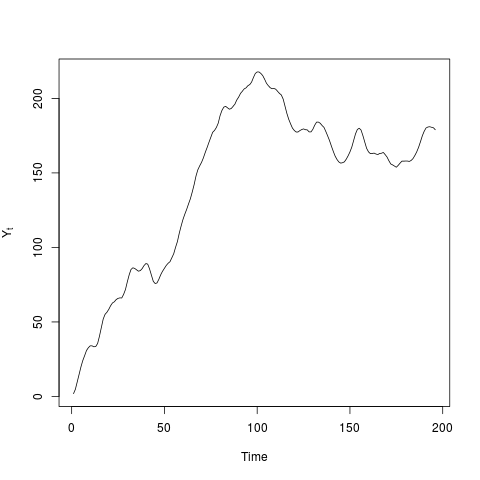
\includegraphics[width=4.0in]{img/arima112nzm.png}

\noindent
\textbf{The Theoretical Model:} 
\[
(\nabla Y_{t} - \mu) = \phi(\nabla Y_{t - 1} - \mu) +  e_{t} + \theta_{1} e_{t - 1} + \theta_{2} e_{t - 2},\ t = 1,2,\ldots
\]

\noindent
\textbf{How to Fit the Model with R:}


\begin{verbatim}
Arima(y, order = c(1,1,2), include.drift = TRUE)
\end{verbatim}




\begin{verbatim}
Series: y 
ARIMA(1,1,2) with drift         

Coefficients:
         ar1     ma1     ma2   drift
      0.7103  0.6555  0.5095  0.8674
s.e.  0.0622  0.0873  0.0732  0.4716

sigma^2 estimated as 0.8019:  log likelihood=-256.47
AIC=522.93   AICc=523.25   BIC=539.3
\end{verbatim}

\noindent
\textbf{The Fitted Model:} 
\[
(\nabla Y_{t} - 0.8674 ) = 0.7103 (\nabla Y_{t - 1} - 0.8674 ) + e_{t} + 0.6555 e_{t - 1} + 0.5095 e_{t - 2},\ t = 1,2,\ldots
\]
that is,
\[
\nabla Y_{t} = 0.2513 + 0.7103 \nabla Y_{t - 1} + e_{t} + 0.6555 e_{t - 1} + 0.5095 e_{t - 2},\ t = 1,2,\ldots
\]
\section*{ARIMA(1,2,1) without drift}
\label{sec-9}


\begin{verbatim}
ydiffdiff <- arima.sim(model = list(ar = 0.9, ma = 0.5), n = 175)
y <- ts(cumsum(cumsum(ydiffdiff)))
\end{verbatim}





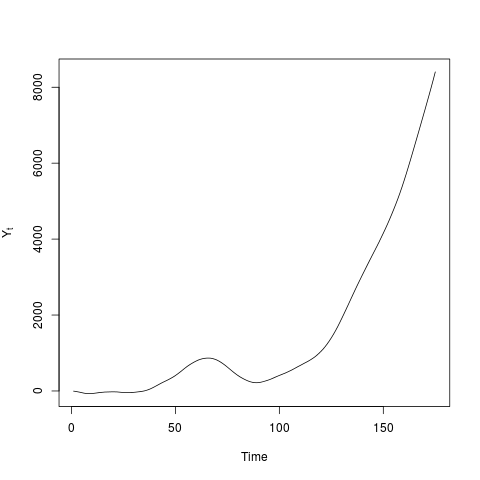
\includegraphics[width=4.0in]{img/arima121zm.png}

\noindent
\textbf{The Theoretical Model:} 
\[
\nabla^{2} Y_{t} = \phi \nabla^{2} Y_{t - 1} + e_{t} + \theta e_{t - 1},\ t = 1,2,\ldots
\]

\noindent
\textbf{How to Fit the Model with R:}


\begin{verbatim}
Arima(y, order = c(1,2,1))
\end{verbatim}




\begin{verbatim}
Series: y 
ARIMA(1,2,1)                    

Coefficients:
         ar1     ma1
      0.9039  0.5756
s.e.  0.0346  0.0666

sigma^2 estimated as 1.002:  log likelihood=-247.12
AIC=500.24   AICc=500.38   BIC=509.7
\end{verbatim}

\noindent
\textbf{The Fitted Model:} 
\[
\nabla^{2} Y_{t} = 0.9039 \nabla^{2} Y_{t - 1} + e_{t} + 0.5756 e_{t - 1},\ t = 1,2,\ldots
\]

\end{document}